\documentclass[../main/main.tex]{subfiles}

% \toggletrue{student}
% \HideSolutionstrue

\raggedbottom

\makeatletter
\renewcommand{\@chapapp}{Induction -- chapitre}
\makeatother

\begin{document}
\setcounter{chapter}{1}

\chapter{Actions mécaniques du champ magnétique}
\label{ch:ind_meca}
\section{Observations expérimentales}
\label{sec:obsexp}
\paragraph*{Aimant}
Pour introduire la notion d'aimant et définir la boussole, nous avons dit qu'une
petite aiguille aimantée s'alignait sur la direction du champ magnétique. Il y a
donc une action mécanique entre aimant et champ.

\begin{figure}[h]
	\centering
	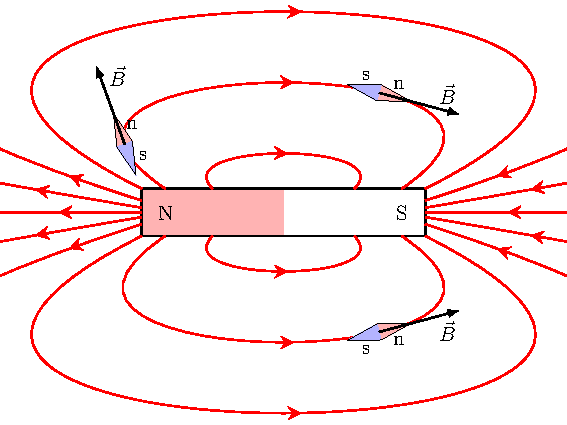
\includegraphics[scale=.8]{aim_ac}
	\label{fig:aim_ac}
\end{figure}

\paragraph*{Rails de \textsc{Laplace}}
Une autre manifestation remarquable est celle des \textbf{rails de
	\textsc{Laplace}}. Soit l'expérience suivante~:
\begin{figure}[h]
	\centering
	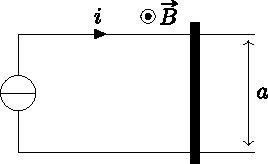
\includegraphics[scale=1]{rlp_1}
	\label{fig:rlp_1}
\end{figure}
On utilise un aimant en U pour créer un champ magnétique uniforme sur une assez
grande partie d'un barreau métallique mobile, posé sur un bout de circuit
électrique. Le barreau permet de ferme le circuit.
\switch{
	\setlist{nosep}
}{
	\setlist{itemsep=5pt}
}
\begin{itemize}[label=$\diamond$, leftmargin=10pt]
	\item \cswitch{white}{
		      Lorsqu'on allume le courant, le barreau se met en mouvement \textbf{vers
			      la gauche}.
	      }
	\item \cswitch{white}{
		      En inversant l'aimant \textbf{ou} en inversant le sens du courant, le
		      mouvement a lieu \textbf{dans l'autre sens}.
	      }
	\item \cswitch{white}{
		      En mettant $\vv{B}$ dans le sens de la tige mobile, il n'y a pas de
		      mouvement.
	      }
\end{itemize}
Ces observations suggèrent l'existence d'une force dépendant du courant et du
champ magnétique, ainsi que de la direction du barreau.

\section{La force de \textsc{Laplace}}
\label{sec:flpl}
\subsection{Densité linéique de la force de \textsc{Laplace}}
\label{ssec:flplliq}
Dans un fil électrique parcouru par un courant, les électrons de conduction sont
en mouvement. Placés dans un champ magnétique, ils subissent la force de
\textsc{Lorentz} $\vv{F} = -e \vv{v}\wedge \vv{B}$~: c'est l'origine de la force
de \textsc{Laplace}. Établissons son expression en fonction de l'intensité
parcourant le circuit.

\paragraph*{Hypothèses de calcul}~
\begin{hide}
	\begin{itemize}[label=$\diamond$, leftmargin=10pt]
		\item On suppose que les électrons sont animés d'une même vitesse $\vv{v} =
			      v \ux$, où $\ux$ désigne la direction du fil\footnote{Cette hypothèse a pour
			      but de simplifier le calcul~: dans la situation réelle, $v$ représente la
			      vitesse \textbf{moyenne} des électrons.}~;
		\item le nombre d'électrons par unité de volume $n$ (en \si{m^{-3}}) est
		      homogène~;
		\item on considère un fil de section $S$ constante.
	\end{itemize}
\end{hide}

\paragraph*{Expression de l'intensité du courant}~
\begin{hide}
	Pendant un intervalle $\dd{t}$, les électrons situés dans un cylindre de
	longueur $v \dd{t}$ en amont de $S$ vont passer à travers la section $S$~: $v
		\dd{t}$ correspond à la distance parcourue par les électrons pendant cet
	intervalle. Ceux qui sont plus loin ne la traversent pas. Dans ce cylindre, il y
	a $\dd{N} = n\times Sv \dd{t}$ électrons, soit une charge $\dd{q} = -e \dd{N} =
		-neSv \dd{t}$. L'intensité du courant est donc
	\[
		i = \dv{q}{t} = -neSv
	\]
\end{hide}

\begin{figure}[h]
	\centering
	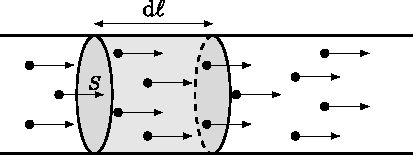
\includegraphics[scale=1]{cyl1}
	\label{fig:cyl1}
\end{figure}

\paragraph*{Expression de la force subie par une section de fil}~
\begin{hide}
	Considérons une section de longueur $\dd{\ell}$ de fil. Dans cette section, il y a
	$n\times S \dd{\ell}$ électrons. Chaque électron subit la force de
	\textsc{Lorentz} $-e \vv{v} \wedge \vv{B}$. La force subie par la section de fil
	est donc
	\begin{align*}
		\dd{\vv{F}} & = -neS \dd{\ell}\vv{v}\wedge \vv{B}
		\\\Lra
		\dd{\vv{F}} & = -neSv (\dd{\ell}\ux)\wedge \vv{B}
	\end{align*}
	En notant $\vv{\dd{\ell}} = \dd{\ell}\ux$ l'élément de déplacement. Alors,
\end{hide}
\begin{tdefi}{Définition, heart}
	\cswitch{white}{
		La force de \textsc{Laplace} subie par un élément de fil de longueur
		$\dd{\ell}$ est
		\[
			\boxed{\dd{\vv{F_{\textsc{Laplace}}}} = i \vv{\dd{\ell}}\wedge \vv{B}}
		\]
		avec $\vv{\dd{\ell}}$ orienté \textbf{dans le sens du courant}.
	}
\end{tdefi}

\subsection{Expression intégrale de la force de \textsc{Laplace}}
\label{ssec:lplint}
Si le champ magnétique est homogène sur un fil rectiligne AC (schéma), alors on
\textbf{intègre} sur la longueur~:
\smallbreak
\noindent
\begin{minipage}[t]{.5\linewidth}
	\cswitch{white}{
		\begin{align*}
			\vv{F_{\textsc{Laplace}}}
			 & = \int_{\rm A}^{\rm B} i \vv{\dd{\ell}}\wedge \vv{B}
			\\\Lra
			\vv{F_{\textsc{Laplace}}}
			 & = i \left( \int_{\rm A}^{\rm C} \vv{\dd{\ell}}\right)\wedge \vv{B}
		\end{align*}
		Avec $\int_{\rm A}^{\rm C} \vv{\dd{\ell}} = \vv{\rm AC}$, on a ainsi
	}
\end{minipage}
\hfill
\begin{minipage}[t]{.5\linewidth}
	~
	%\vspace*{-20pt}
	\begin{center}
		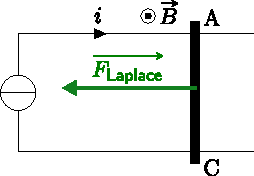
\includegraphics[scale=1]{rlp_2}
		\label{fig:rlp_2}
	\end{center}
\end{minipage}

\begin{tdefi}{Définition, heart}
	\cswitch{white}{
		La force de \textsc{Laplace} qui s'exerce sur une barre conductrice AC
		traversée par un courant $i$ et placée dans un champ magnétique
		\textbf{uniforme} et \textbf{stationnaire} $\vv{B}$ s'applique en son
		milieu et vaut~:
		\[
			\boxed{\vv{F_{\textsc{Laplace}}} = i \vv{\rm AC}\wedge \vv{B}}
		\]
		où $i$ est orienté \textbf{selon le sens du vecteur} $\vv{\rm AC}$.
	}
\end{tdefi}
\begin{rexem}{Remarques}
	\begin{minipage}[t]{.68\linewidth}
		\begin{enumerate}
			\item On peut orienter la force selon la règle de la main droite, version
			      «~trois doigts~»~:
			      \begin{itemize}[label=$\diamond$, leftmargin=20pt]
				      \item \cswitch{white}{
					            la force sur le pouce («~le pouce pousse~»)~;
				            }
				      \item \cswitch{white}{
					            l'\textbf{in}tensité sur l'\textbf{in}dex~;
				            }
				      \item \cswitch{white}{
					            le champ \textbf{ma}gnétique sur le \textbf{ma}jeur.
				            }
			      \end{itemize}
			\item Cette expression permet d'obtenir la dimension de $B$ en fonction des
			      dimensions fondamentales~:
			      \cswitch{white}{
				      \[
					      B = \frac{F}{\ell i} \Lra [B]
					      = \frac{\rm M \cdot L \cdot T^{-2}}{\rm L \cdot I}
					      = \mathrm{M \cdot T^{-2} \cdot I^{-1}}
				      \]
			      }
		\end{enumerate}
	\end{minipage}
	\hfill
	\begin{minipage}[t]{.30\linewidth}
		~
		\vspace*{-20pt}
		\begin{center}
			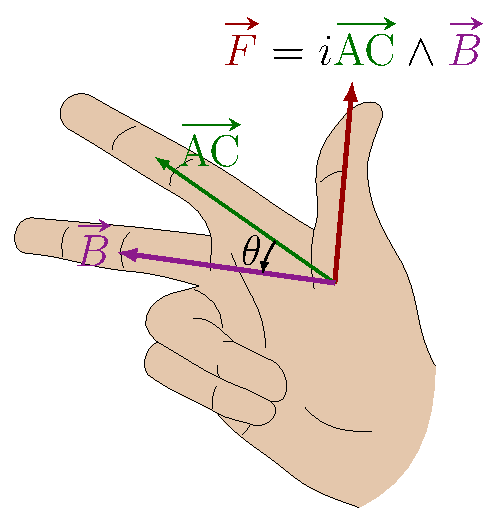
\includegraphics[width=\linewidth]{righthand_laplace}
			\label{fig:ra_lpl}
		\end{center}
	\end{minipage}
	\begin{enumerate}[start=3]
		\item L'ordre de grandeur de cette force pour un fil de \SI{5}{cm} dans un
		      champ de \SI{0.1}{T} parcouru par une intensité de \SI{1}{A} est~:
		      \cswitch{white}{
			      \[
				      \boxed{\norm{\vv{F_{\textsc{Laplace}}}} = i \ell B = \SI{5}{mN}}
			      \]
		      }
		\item La puissance de la force de \textsc{Laplace} correspondante est~:
		      \cswitch{white}{
		      \[
			      \boxed{
			      \mathcal{P}_{\textsc{Laplace}}
			      = \left( i \vv{\rm AC}\wedge \vv{B} \right) \cdot \vv{v}}
		      \]
		      }
		      \switch{
			      Ainsi, alors que la force de magnétique de \textsc{Lorentz} était de
			      puissance nulle sur \textbf{1 électron}, ça n'est pas le cas de la force
			      de \textsc{Laplace} qui s'applique sur un solide conducteur~: dans ce
			      cas, \textbf{un champ magnétique peut accélérer le système}.
		      }{
			      \vspace{-10pt}
		      }
	\end{enumerate}
\end{rexem}

\section{Le couple des actions de \textsc{Laplace}}
\label{sec:lplcpl}

\subsection{Spire rectangulaire plongée dans un champ constant}
\label{ssec:lplcplspire}
On commence par un cas particulier~: une spire rectangulaire dans un champ
constant.
\begin{figure}[h!]
	\centering
	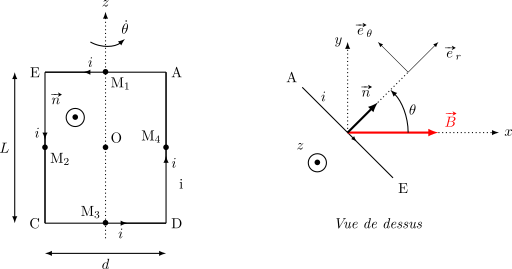
\includegraphics[scale=.8]{spir1}
	\label{fig:spir1}
\end{figure}
\switch{
	\setlist{nosep}
}{
	\setlist{nosep}
}
\begin{itemize}[label=$\diamond$, leftmargin=10pt]
	\item On considère un cadre rectangulaire AECD parcouru par un courant $i$. Ce
	      cadre peut tourner autour de l'axe $(\Or z)$.
	\item On impose un champ magnétique uniforme $\vv{B} = B\ux$. On note $\theta$
	      l'angle entre $\vv{B}$ et la normale au cadre, orientée \textbf{dans le sens
		      de} $i$. On note cette normale $\vv{n}$.
\end{itemize}
\paragraph*{Résultante des forces}~
\begin{hide}
	Il s'agit d'additionner les différentes forces de \textsc{Laplace} subies par
	chacun des côtés de la spire rectangulaire. Sur le côté AE par exemple~:
	\[
		\vv{F_{\textsc{Lap}, \rm AE}} = i \vv{\rm AE}\wedge \vv{B}
	\]
	La résultante est donc
	\begin{align*}
		\sum \vv{F_{\rm Lap}}         & =
		i \vv{\rm AE}\wedge \vv{B} +
		i \vv{\rm EC}\wedge \vv{B} +
		i \vv{\rm CD}\wedge \vv{B} +
		i \vv{\rm DA}\wedge \vv{B}
		\\\Lra
		\sum \vv{F_{\rm Lap}}         & =
		i \left( \vv{\rm AE} + \vv{\rm EC} + \vv{\rm CD} + \vv{\rm DA} \right)\wedge
		\vv{B}
		\\\Lra
		\Aboxed{\sum \vv{F_{\rm Lap}} & = \vv{0}}
	\end{align*}
\end{hide}

\begin{rexem}{Remarque}
	Tant que le champ magnétique est homogène, alors peu importe le circuit fermé,
	on aura
	\[
		\oint_{\mathcal{C}}^{} i \vv{\dd{\ell }}\wedge \vv{B} =
		i \left( \oint_{\mathcal{C}} \vv{\dd{\ell }} \right)\wedge \vv{B} = \vv{0}
	\]
\end{rexem}
\paragraph*{Couple des forces} On a la force agissant sur le côté $\vv{\rm
		AE}$~:
\begin{hide}
	\begin{align*}
		\vv{F_{\rm Lap,AE}}
		 & = i \vv{\rm AE}\wedge \vv{B}
		\\
		 & = i (-d \cos{\theta}\uy + d\sin{\theta}\ux)\wedge \vv{B}
		\\
		 & = idB\cos{\theta}\uz
	\end{align*}
	La force s'exerce de façon constante tout le long de la spire, donc son point
	d'application est $\Mr_1$, qui est un point de l'axe de rotation. Ainsi,
	\textbf{son moment est nul}~:
	\[
		\boxed{\Mc_z \left( \vv{F_{\rm Lap,AE}} \right) =
			\left( \vv{\rm OM_1}\wedge \vv{B} \right)\cdot \uz
			= 0}
	\]
\end{hide}
\noindent
Sur le côté $\vv{\rm EC}$~:
\begin{hide}
	\begin{align*}
		\vv{F_{\rm Lap,EC}}
		 & = i \vv{\rm EC}\wedge \vv{B}
		\\
		 & = i (-L\uz)\wedge B\ux
		\\
		 & = -iLB\uy
	\end{align*}
	Le point d'application est $\Mr_2$, donc~:
	\begin{align*}
		\Mc_z \left(\vv{F_{\rm Lap,EC}}\right)
		 & = \left(\vv{\rm OM_2}\wedge \vv{F_{\rm Lap,EC}}\right)\cdot \uz
		\\
		 & = \left(
		\left(
			-\frac{d}{2}\cos{\theta}\uy +
			\frac{d}{2}\sin{\theta}\ux
			\right)\wedge -iLB\uy
		\right)\cdot \uz
		\\\Lra
		\Aboxed{\Mc_z (\vv{F_{\rm Lap,EC}})
		 & = -iLB \frac{d}{2}\sin{\theta}}
	\end{align*}
\end{hide}
\noindent
La force agissant sur le côté $\vv{\rm CD}$ s'applique en $\Mr_3$, qui est sur
l'axe de rotation, donc immédiatement~:
\begin{hide}
	\[
		\boxed{\Mc_z \left( \vv{F_{\rm Lap,CD}} \right) = 0}
	\]
\end{hide}
\noindent
Et enfin sur le côté $\vv{\rm DA}$~:
\begin{hide}
	\begin{align*}
		\vv{F_{\rm Lap,DA}}
		 & = i \vv{\rm DA}\wedge \vv{B}
		\\
		 & = i (L\uz)\wedge B\ux
		\\
		 & = iLB\uy
	\end{align*}
	Le point d'application est $\Mr_4$, donc~:
	\begin{align*}
		\Mc_z \left( \vv{F_{\rm Lap,DA}} \right)
		 & = \left( \vv{\rm OM_4} \wedge \vv{F_{\rm Lap,DA}} \right)\cdot \uz
		\\
		 & = \left(
		\left(
			\frac{d}{2}\cos{\theta}\uy
			- \frac{d}{2}\sin{\theta}\ux
			\right)\wedge iLB\uy
		\right)\cdot \uz
		\\\Lra
		\Aboxed{\Mc_z \left( \vv{F_{\rm Lap,DA}} \right)
		 & = -iLB \frac{d}{2}\sin{\theta}}
	\end{align*}
\end{hide}
\noindent
En sommant tous ces moments, on trouve donc~:
\begin{hide}
	\[
		\Mc_{\mathrm{Lap},z} = -idLB\sin{\theta}
	\]
\end{hide}
\noindent
Avec le moment magnétique de la spire $\vv{\mu} = iS \vv{n}$, on trouve~:
\begin{hide}
	\begin{align*}
		\vv{\mu}\wedge \vv{B}
		 & = iS (\cos{\theta}\ux+\sin{\theta}\uy \wedge B\ux)
		\\
		 & = -iSB\sin{\theta}\uz
		\\
		 & = -iLdB\sin{\theta}\uz
	\end{align*}
	Ainsi,
\end{hide}
\begin{tprop}{Moment des forces de \textsc{Laplace}, heart}
	\cswitch{white}{%
		Un circuit ou un aimant de moment magnétique $\vv{\mu}$ plongé dans un champ
		\textbf{uniforme} et \textbf{stationnaire} $\vv{B}$ subit un \textbf{couple
			magnétique}, issu du moment des forces de \textsc{Laplace} par rapport à un
		axe $\uz$ tel que~:
		\[
			\boxed{\Mc_{\mathrm{Lap},z} = \left( \vv{\mu}\wedge \vv{B} \right)\cdot \uz}
		\]
		D'où la \textbf{puissance} pour le système en rotation~:
		\[
			\boxed{\Pc_{\rm Lap} = \Mc_{\rm Lap,z}\cdot \w = \left( \Mcf_{\rm
					Lap}\cdot \uz \right)\w}
		\]
		avec $\w$ la vitesse angulaire de rotation autour de l'axe $z$.
	}
\end{tprop}

\subsection{Effet sur un aimant}
\label{ssec:lplcplaim}

Par analogie avec la spire, on peut dire qu'un moment magnétique soumis à un
champ magnétique génère un couple de forces, de moment résultant~:
\smallbreak
\noindent
\begin{minipage}[t]{.5\linewidth}
	\[
		\Mc_z = \left( \vv{m}\wedge \vv{B} \right)\cdot \uz
	\]
\end{minipage}
\hfill
\begin{minipage}[t]{.5\linewidth}
	~
	\vspace*{-30pt}
	\begin{center}
		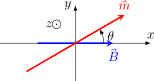
\includegraphics[scale=1]{aim_cpl}
		\label{fig:aim_cpl}
	\end{center}
\end{minipage}
\begin{rexem}{Application}
	\begin{enumerate}
		\item Exprimer le couple de \textsc{Laplace} subit par $\vv{m}$ en fonction
		      de $\tt$.
		\item En déduire les positions d'équilibre de $\vv{m}$.
		\item En étudiant dans quel sens le couple de \textsc{Laplace} tend à faire
		      tourner $\vv{m}$ en cas de petites perturbations, déterminer laquelle des
		      deux positions d'équilibre est stable, et laquelle est instable.
	\end{enumerate}
	\tcblower
	\cswitch{white}{
		\begin{enumerate}
			\item On a
			      \begin{align*}
				      \vv{m} & = m \left( \cos{\theta}\ux + \sin{\theta}\uy \right)
				      \\
				      \vv{B} & = B_0\ux
			      \end{align*}
			      D'où
			      \[
				      \boxed{\Mcf_z = -mB_0\sin{\theta}\uz}
			      \]
			      Ce qui fait tourner le système autour de l'axe $z$.
			\item On est à l'équilibre si la somme des forces et la somme des moments
			      sont nulles. Avec uniquement le couple magnétique, on a bien une
			      résultante nulle~: on a donc équilibre si $\Mcf_z = \vv{0}$, soit
			      \begin{align*}
				      \sin{\tt_{\rm eq}} & = 0
				      \\\Lra
				      \tt_{\rm eq}       & = 0
				      \\\qqou
				      \tt_{\rm eq}       & = \pi
			      \end{align*}
			\item
			      \begin{itemize}
				      \item En $\tt_{\rm eq} = \pi$, une petite déviation vers le haut
				            donne un mouvement de rotation dans le sens horaire, qui écarte
				            donc l'aimant de sa position d'équilibre~: il est
				            \textbf{instable}.
				      \item À l'inverse, en $\tt_{\rm eq} = 0$, une petite
				            déviation vers le haut donne un mouvement de rotation dans
				            le sens direct, le ramenant à sa position d'équilibre~: il
				            est \textbf{stable}.
			      \end{itemize}
		\end{enumerate}
	}
\end{rexem}

La dynamique de la rotation de l'aimant est alors équivalente à celle du pendule
pesant~! En effet, en appliquant le théorème du moment cinétique à l'aimant~:
\[
	\dv{\Lc_z}{t} = J\tpp = \sum \Mc_z
\]
avec $J$ le moment d'inertie par rapport à l'axe de rotation. Or,
d'après ce qui précède,
\begin{align*}
	\sum \Mc_z                              & = -mB\sin{\theta}
	\\\Lra
	J\tpp                                   & = -mB\sin{\theta}
	\\\Lra
	\Aboxed{\tpp + \frac{mB}{J}\sin{\theta} & = 0}
\end{align*}
qui est bien l'équation du pendule.
\begin{tror}{Conclusion, hand}
	\cswitch{white}{
		Du fait des petites vibrations (qui rendent la position $\theta=\pi$ non
		durable) et des frottements qui arrêtent sa course, \textbf{un aimant tend à
			s'aligner sur le champ magnétique}, et ce d'autant plus vite que le champ
		$\vv{B}$ est intense.
	}
\end{tror}
En effet, au voisinage de
la position d'équilibre, on a $\sin{\theta} \sim \theta$, d'où
\[
	\tpp + \frac{mB}{J}\theta = 0
\]
qui est l'équation d'un \textbf{oscillateur harmonique}, de période propre~:
\[
	T_0 = 2\pi \sqrt{\frac{J}{mB}}
\]

\subsection{Boussole sur Terre}
\label{ssec:boussoleterre}

\begin{minipage}[t]{.5\linewidth}
	On peut donc pleinement expliquer l'alignement d'une boussole à la surface de la
	Terre, toujours en modélisant son champ magnétique par un aimant~: l'aiguille
	aimantée de moment magnétique $\vv{\mu}$ s'oriente spontanément sur le champ
	magnétique terrestre.
	\bigbreak
	On notera bien que dans ce cas, la boussole pointe bien
	vers le Nord géographique, mais qu'il correspond au Sud magnétique de la Terre.
\end{minipage}
\hfill
\begin{minipage}[t]{.5\linewidth}
	~
	\vspace*{-40pt}
	\begin{center}
		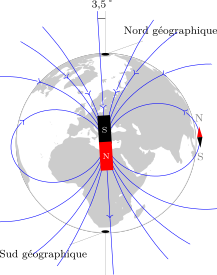
\includegraphics[scale=1]{boussole_terre}
		\label{fig:bterre}
	\end{center}
\end{minipage}

\section{Effet moteur d'un champ magnétique tournant}
\label{sec:btourne}
Si un aimant a tendance à s'orienter sur un champ magnétique, on peut utiliser
ce couple pour forcer la rotation continue d'un aimant grâce à un \textbf{champ
	tournant}~: c'est le principe du \textbf{moteur synchrone}.
\begin{tdefi}{Définition}
	\begin{minipage}[c]{.6\linewidth}
		\begin{center}
			\cswitch{white}{
				Un champ tournant est un champ de norme constante, mais dont la direction
				tourne à vitesse angulaire constante. Par le couple de \textsc{Laplace},
				un aimant soumis à ce champ tournera en régime stationnaire à la même
				vitesse angulaire $\w$.
			}
		\end{center}
	\end{minipage}
	\hfill
	\begin{minipage}[c]{.4\linewidth}
		~
		\begin{center}
			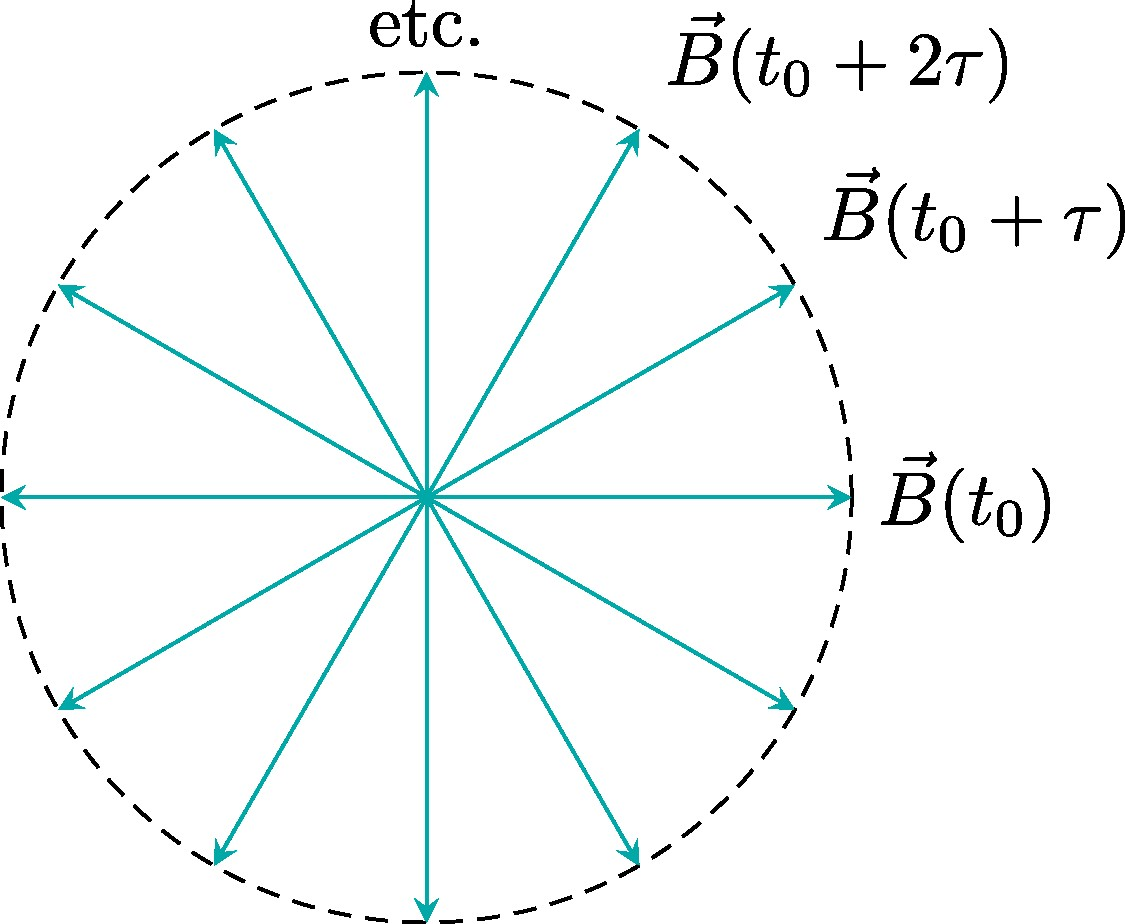
\includegraphics[scale=1]{btourn1}
			\captionof{figure}{Champ magnétique tournant.}
			\label{fig:btourn1}
		\end{center}
	\end{minipage}
\end{tdefi}
\noindent
\begin{minipage}[t]{.5\linewidth}
	Pour réaliser un champ tournant, on peut utiliser deux bobines identiques, de
	courants déphasés de $\pi/2$~:
	\begin{align*}
		i_1(t) & = I_0\cos{\wt}
		\\\qqet
		i_2(t) & = I_0\cos{\wt-\pi/2} = I_0\sin{\wt}
	\end{align*}
	Ainsi, proche de l'axe des bobines on aura des champs
	\begin{gather*}
		\vv{B_1}(t) = k I_0\cos{\wt}\,\ux
		\qqet
		\vv{B_2}(t) = k I_0\sin{\wt}\,\uy
	\end{gather*}
	Soit, par somme~:
	\cswitch{white}{
		\[
			\boxed{\vv{B} = k I_0 (\cos{\wt}\ux + \sin{\wt}\uy) = k I_0\ur}
		\]
	}
	qui est bien un champ tournant.
\end{minipage}
\hfill
\begin{minipage}[t]{.5\linewidth}
	~
	\begin{center}
		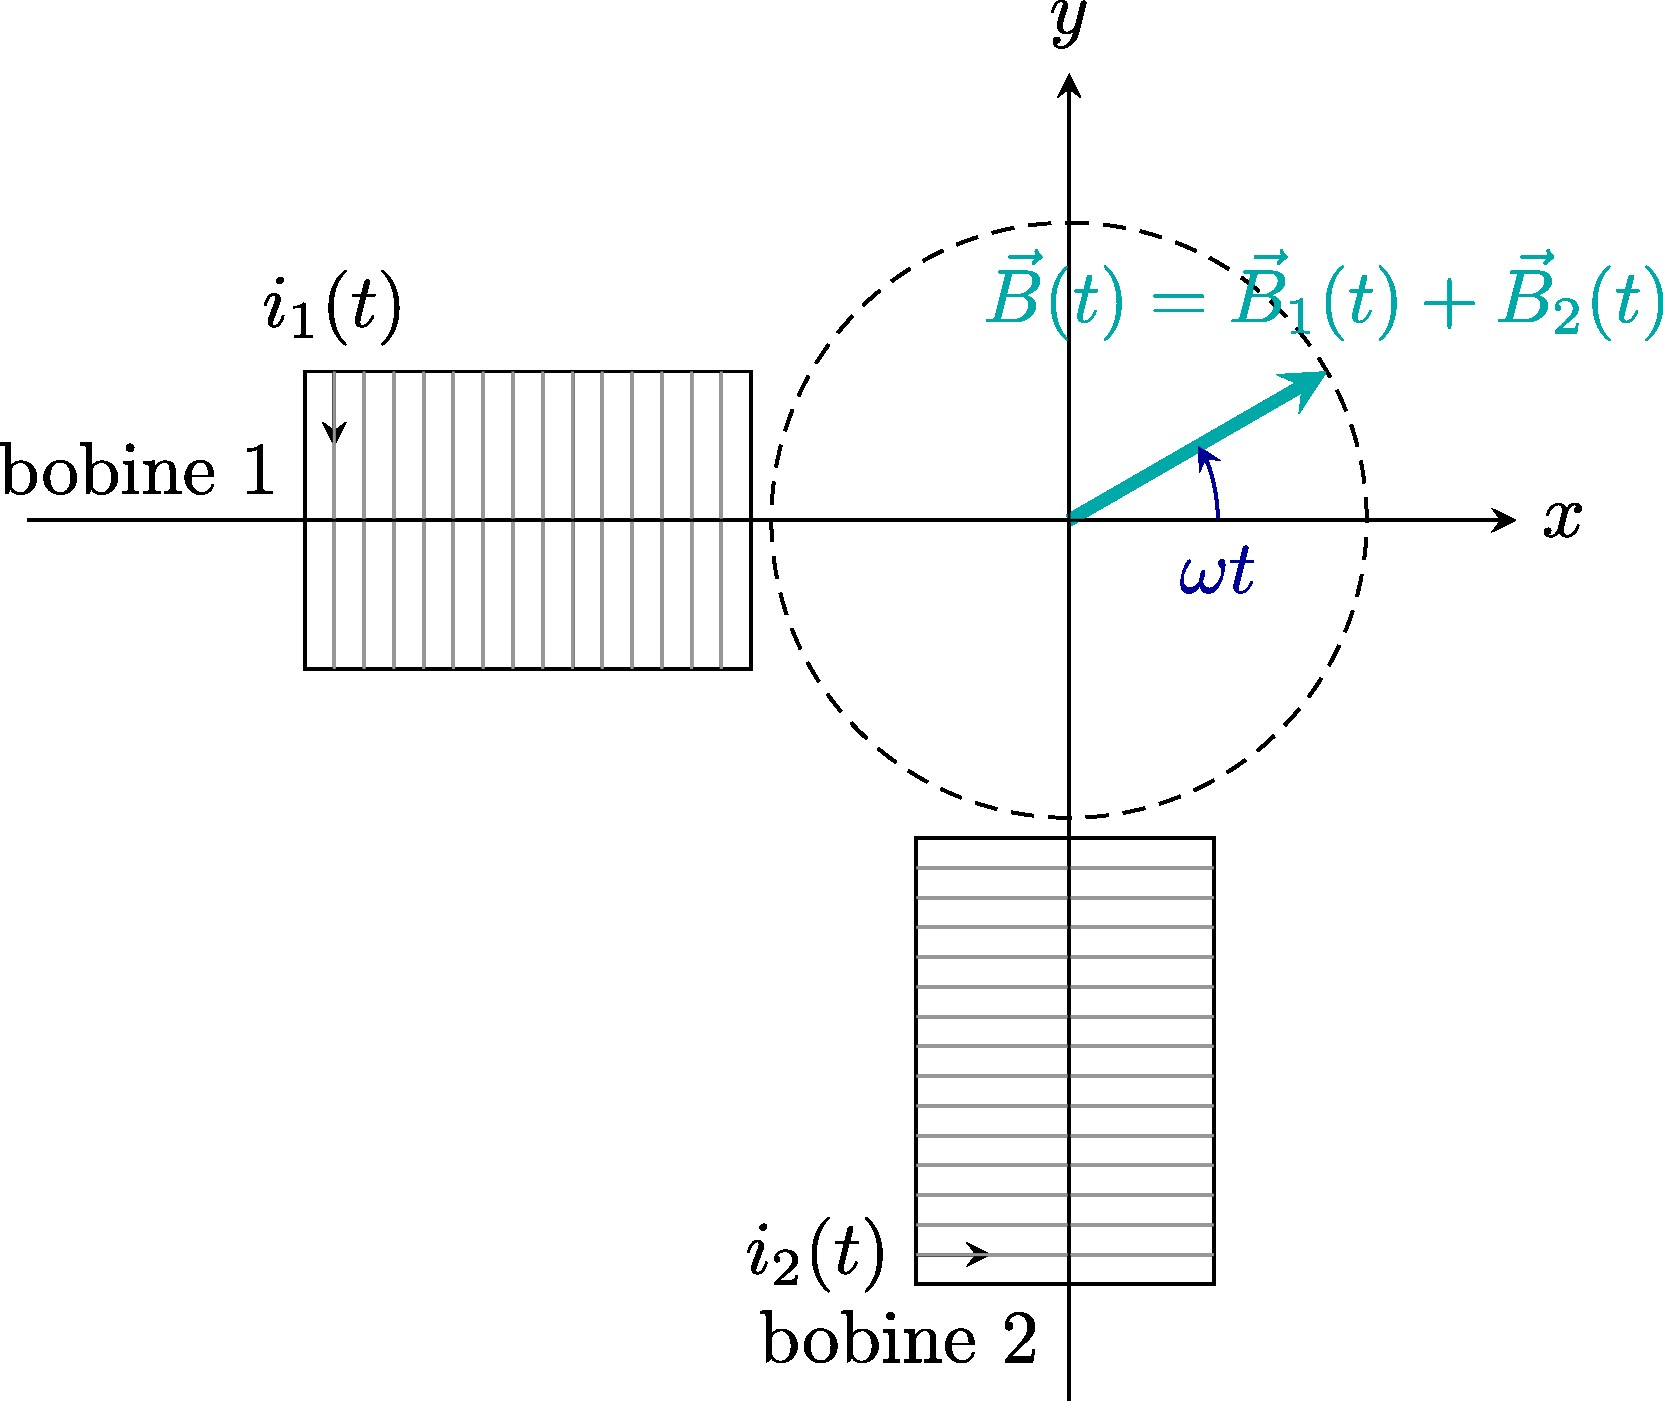
\includegraphics[scale=1]{btourn2}
		\label{fig:btourn2}
	\end{center}
\end{minipage}
Il est également possible de faire un champ tournant à l'aide de trois bobines,
décalées de $2\pi/3$~: c'est ce qu'on appelle un courant \textbf{triphasé}, et
c'est ce qui est utilisé dans le transport d'électricité de manière
industrielle.

\end{document}
